\documentclass[12pt, a4paper, oneside]{ctexart}
\usepackage{amsmath, amsthm, amssymb, bm, color, graphicx, geometry, mathrsfs,extarrows, braket, booktabs, array}
\usepackage[colorlinks,linkcolor=red,anchorcolor=blue,citecolor=blue,urlcolor=blue,menucolor=black]{hyperref}
%%%% 设置中文字体 %%%%
\setCJKmainfont{方正新书宋_GBK.ttf}[BoldFont=方正小标宋_GBK, ItalicFont=方正楷体_GBK]
%%%% 设置英文字体 %%%%
\setmainfont{Times New Roman}
\setsansfont{Calibri}
\setmonofont{Consolas}

\linespread{1.4}
%\geometry{left=2.54cm,right=2.54cm,top=3.18cm,bottom=3.18cm}
\geometry{left=1.84cm,right=1.84cm,top=2.18cm,bottom=2.18cm}
\newcounter{problem}  % 问题序号计数器
\newenvironment{problem}[1][]{\stepcounter{problem}\par\noindent\textbf{题目\arabic{problem}. #1}}{\smallskip\par}
\newenvironment{solution}[1][]{\par\noindent\textbf{#1解答. }}{\smallskip\par}  % 可带一个参数表示题号\begin{solution}{题号}
\newenvironment{note}{\par\noindent\textbf{注记. }}{\smallskip\par}

%%%% 图片相对路径 %%%%
\graphicspath{{figure/}} % 当前目录下的figure文件夹, {../figure/}则是父目录的figure文件夹
\setlength{\abovecaptionskip}{-0.2cm}  % 缩紧图片标题与图片之间的距离
\setlength{\belowcaptionskip}{0pt} 

\everymath{\displaystyle} % 默认全部行间公式
\DeclareMathOperator*\uplim{\overline{lim}} % 定义上极限 \uplim_{}
\DeclareMathOperator*\lowlim{\underline{lim}} % 定义下极限 \lowlim_{}
\DeclareMathOperator*{\argmax}{arg\,max}  % \argmin
\DeclareMathOperator*{\argmin}{arg\,min}  % \argmax
\let\leq=\leqslant % 将全部leq变为leqslant
\let\geq=\geqslant % geq同理

%%%% 一些宏定义 %%%%
\def\bd{\boldsymbol}        % 加粗(向量) boldsymbol
\def\disp{\displaystyle}    % 使用行间公式 displaystyle(默认)
\def\tsty{\textstyle}       % 使用行内公式 textstyle
\def\sign{\text{sign}}      % sign function
\def\wtd{\widetilde}        % 宽波浪线 widetilde
\def\R{\mathbb{R}}          % Real number
\def\N{\mathbb{N}}          % Natural number
\def\Z{\mathbb{Z}}          % Integer number
\def\Q{\mathbb{Q}}          % Rational number
\def\C{\mathbb{C}}          % Complex number
\def\N{\mathbb{N}}          % Natural number
\def\Z{\mathbb{Z}}          % Integer number
\def\E{\mathbb{E}}          % Exception
\def\var{\text{Var}}        % Variance
\def\bias{\text{bias}}      % bias
\def\d{\mathrm{d}}          % differential operator
\def\e{\mathrm{e}}          % Euler's number
\def\i{\mathrm{i}}          % imaginary number
\def\re{\mathrm{Re}}        % Real part
\def\im{\mathrm{Im}}        % Imaginary part
\def\res{\mathrm{Res}}      % Residue
\def\L{\mathcal{L}}         % Loss function
\def\wdh{\widehat}          % 宽帽子 widehat
\def\ol{\overline}          % 上横线 overline
\def\ul{\underline}         % 下横线 underline
\def\add{\vspace{1ex}}      % 增加行间距
\def\del{\vspace{-1.5ex}}   % 减少行间距

%%%% 定理类环境的定义 %%%%
\newtheorem{theorem}{定理}

%%%% 基本信息 %%%%
\newcommand{\RQ}{\today} % 日期
\newcommand{\km}{数理统计} % 科目
\newcommand{\bj}{强基数学002} % 班级
\newcommand{\xm}{吴天阳} % 姓名
\newcommand{\xh}{2204210460} % 学号
\newcommand{\id}{50} % 序号

\begin{document}

%\pagestyle{empty}
\pagestyle{plain}
\vspace*{-15ex}
\centerline{\begin{tabular}{*6{c}}
    \parbox[t]{0.25\linewidth}{\begin{center}\textbf{日期}\\ \large \textcolor{blue}{\RQ}\end{center}} 
    & \parbox[t]{0.2\linewidth}{\begin{center}\textbf{科目}\\ \large \textcolor{blue}{\km}\end{center}}
    & \parbox[t]{0.2\linewidth}{\begin{center}\textbf{班级}\\ \large \textcolor{blue}{\bj}\end{center}}
    & \parbox[t]{0.1\linewidth}{\begin{center}\textbf{姓名}\\ \large \textcolor{blue}{\xm}\end{center}}
    & \parbox[t]{0.15\linewidth}{\begin{center}\textbf{学号}\\ \large \textcolor{blue}{\xh}\end{center}}
    & \parbox[t]{0.1\linewidth}{\begin{center}\textbf{序号}\\ \large \textcolor{blue}{\id}\end{center}}
     \\ \hline
\end{tabular}}
\begin{center}
    \zihao{3}\textbf{第四次作业}
\end{center}\vspace{-0.2cm}
\begin{problem}[(22)]
    设$X_1,\cdots,X_n$是来满足参数为$\theta$的Bernoulli分布的随机样本.

    (1). 求解$\theta(1-\theta)$的C-R下界.

    (2). 若$\theta(1-\theta)$的UMVUE存在,对其进行求解.
\end{problem}
\begin{solution}
    (1). Bernoulli分布的概率密度函数为$f(x;\theta) = \theta^x(1-\theta)^{1-x}I_{\{0,1\}}(x)$,则
    \begin{equation*}
        \frac{\partial}{\partial\theta}(\log\theta^x(1-\theta^x)) = \frac{x}{\theta}-\frac{1-x}{1-\theta},\quad \frac{\partial^2}{\partial\theta^2}(\log\theta^x(1-\theta)^{1-x}) = -\frac{x}{\theta^2}-\frac{1-x}{(1-\theta)^2},
    \end{equation*}
    则Fisher信息量为$I(\theta) = -\E\left[\frac{\partial^2}{\partial\theta^2}(\log\theta^x(1-\theta)^{1-x})\right] = \frac{1}{(1-\theta)^2}+\left(\frac{1}{\theta^2}-\frac{1}{(1-\theta)^2}\right)\theta = \frac{1}{\theta(1-\theta)}$.\add 于是$\theta(1-\theta)$的C-R下界为$\frac{(1-2\theta)^2}{n\frac{1}{\theta(1-\theta)}} = \frac{(1-2\theta)^2\theta(1-\theta)}{n}$.\add

    (2). 由于$f(x;\theta) = (1-\theta) I_{\{0,1\}}(x)\exp\left\{x\log\frac{\theta}{1-\theta}\right\}$,令$a(\theta) = 1-\theta, b(x) = I_{\{0,1\}}(x),c(\theta) = \log\frac{\theta}{1-\theta},d(x) =x$,则该分布属于指数族,于是$\sum_{i=1}^nX_i$为完备的充分统计量,令$Y = \sum_{i=1}^nX_i,\ Z = \left(\sum_{i=1}^nX_i\right)^2$,由于
    \begin{equation*}
        \E(Y) = n\theta,\ \E(Z) = \E\left[\sum_{i=1}^nX_i^2+2\sum_{1\leq i < j\leq n}X_iX_j\right] = n\theta+n(n-1)\theta^2 = n(n-1)\left(\frac{\theta}{n-1}+\theta^2\right).
    \end{equation*}
    则$\E\left[\frac{Y}{n}\right] = \theta,\ \E\left[\frac{z}{n(n-1)}-\frac{Y}{n(n-1)}\right]=\theta^2$,于是
    \begin{equation*}
        \theta(1-\theta) = \E\left[\frac{Y}{n}\right]-\E\left[\frac{z}{n(n-1)}-\frac{Y}{n(n-1)}\right] = \E\left[\frac{Y}{n-1}-\frac{Z}{n(n-1)}\right],
    \end{equation*}
    由于$\frac{1}{n-1}\sum_{i=1}^nX_i-\frac{1}{n(n-1)}\left(\sum_{i=1}^nX_i\right)^2$是关于完备充分统计量$Y$的函数,\add 且是$\theta(1-\theta)$的无偏估计,所以它是$\theta(1-\theta)$的UMVUE.\add
\end{solution}
\begin{problem}[(24)]
    设$X_1,\cdots,X_n$是来自$\theta x^{\theta-1}I_{(0,1)}(x),\ (\theta > 0)$的随机样本,

    (1). 求解$\mu = \theta/(1+\theta)$的MLE.

    (2). 求解一个充分统计量,并验证其完备性. 判断$\sum_{i=1}^nX_i$是否是充分统计量?

    (3). 是否存在一个关于$\theta$的函数,使得其存在无偏估计且方差满足C-R下界?

    (4). 求解$\theta,1/\theta, \mu=\theta/(1+\theta)$的UMVUE.
\end{problem}
\begin{solution}
    (1). 只需求解$\theta$的MLE:$\L(\theta) = \prod_{i=1}^n\theta x_i^{\theta-1}I_{(0,1)}(x_i)$,由
    \begin{equation*}
        \frac{\partial}{\partial \theta}\log\L(\theta) = \frac{\partial}{\partial \theta}\left(n\log\theta+\sum_{i=1}^n(\theta-1)\log(x_i)+\sum_{i=1}^n\log I_{(0,1)}(x_i)\right) = \frac{n}{\theta}+\sum_{i=1}^n\log(x_i) = 0
    \end{equation*}
    可得$\theta$的MLE为$\hat{\theta} = -\frac{n}{\sum_{i=1}^n\log(x_i)}$. 则$\mu$的MLE为
    \begin{equation*}
        \hat{\mu} = \frac{\hat{\theta}}{1-\hat{\theta}} = \frac{n}{n-\sum_{i=1}^n\log(x_i)}.
    \end{equation*}
    
    (2). 由于$f(x;\theta) = \theta x^{\theta-1}I_{(0,1)}(x) = \theta I_{(0,1)}(x)\exp\{(\theta-1)\log x\}$,令$a(\theta) = \theta,\ b(x)  = I_{(0,1)}(x),$\\$c(\theta) = \theta-1,\ d(x) = \log x$,于是该分布属于指数族,则$\sum_{i=1}^nd(x_i) = \sum_{i=1}^n\log x_i$是一个完备的充分统计量. 由于$\sum_{i=1}^nX_i$不满足因子分解定理,所以不是充分统计量.

    (3). 由于$f_{-\log X}(x) = f_X(\e^{-x})\e^{-x} = \theta\e^{-(\theta-1)x}\e^{-x}I_{(0,1)}(\e^{-x})=\theta\e^{-\theta x}I_{(0,\infty)}(x)$. \add 于是$-\log X\sim \text{Exp}(\theta)$. 令$T = -\frac{1}{n}\sum_{i=1}^n\log X_i$,则$nT\sim\Gamma(n,\theta) \Rightarrow \E(T) = \frac{1}{\theta}$. 则$T$是$\frac{1}{\theta}$的无偏估计,且
    \begin{equation*}
        \sum_{i=1}^n\frac{\partial}{\partial\theta}\log f(x_i;\theta) = \sum_{i=1}^n\frac{\partial}{\partial\theta}(\log\theta+(\theta-1)\log x)=\frac{n}{\theta}+\sum_{i=1}^n\log x_i= -n\left(T-\frac{1}{\theta}\right)
    \end{equation*}
    所以C-R方程取到等号,故$T=-\frac{1}{n}\sum_{i=1}^n\log X_i$取到$\frac{1}{\theta}$的C-R下界.

    (4). 由第三小问可知,$-\frac{1}{n}\sum_{i=1}^n\log X_i$是$\frac{1}{\theta}$的UMVUE.

    做待定系数,令$\frac{c}{-\sum_{i=1}^n\log X_i}$是$\theta$的无偏估计,记$Y = -\sum_{i=1}^n\log X_i$,则
    \begin{align*}
        \E\left[\frac{c}{-\sum_{i=1}^n\log X_i}\right] =&\ \int_0^\infty\frac{c}{y}\frac{\theta^n}{\Gamma(n)}y^{n-1}\e^{-\theta y}\,\d y
        = \frac{c\theta^n}{\Gamma(n)}\cdot\frac{\Gamma(n-1)}{\theta^{n-1}} = \frac{c}{n-1}\theta,
    \end{align*}
    所以$c = n-1$,故$\frac{n-1}{-\sum_{i=1}^n\log X_i}$是$\theta$的UMVUE.
    
    $\theta(1-\theta)$的一个无偏估计为$X_1$,可以得到$\E\left[X_1\biggl|-\sum_{i=1}^n\log X_i\right]=\frac{n-1}{s}\int_0^1(1+\frac{\log x}{s})^{n-2}\,\d x$,但是该积分不会计算,就没写了(应该可以换元后凑Gamma分布得到积分结果).\add
\end{solution}
\begin{problem}[(29)]
    设$X_1,\cdots,X_n$是来自$N(\theta,1)$的随机样本.

    (1). 分别求解关于$\theta, \theta^2, P(X>0)$的C-R下界.

    (2). 当$n=1$时,是否存在关于$\theta^2$的无偏估计?若存在,求解之.

    (3). 是否存在关于$P(X>0)$的无偏估计?若存在,求解之.

    (4). 求解$P(X>0)$的MLE.

    (5). 是否存在关于$\theta^2$的UMVUE.若存在,求解之.

    (6). 是否存在关于$P(X>0)$的UMVUE.若存在,求解之.\add
\end{problem}
\begin{solution}
    (1). $N(\theta,1)$的概率密度函数为$f(x;\theta) = \frac{1}{\sqrt{2\pi}}\exp\left\{-\frac{(x-\theta)^2}{2}\right\}$,则
    \begin{equation*}
        \frac{\partial}{\partial\theta}\log f(x;\theta) = \frac{\partial}{\partial\theta}\left(-\frac{\log 2\pi}{2}-\frac{(x-\theta)^2}{2}\right) = x-\theta,
    \end{equation*}
    Fisher信息量为$I(\theta) = \E\left[\frac{\partial}{\partial\theta}\log f(x;\theta)\right]^2 = \E[x^2-2\theta x+\theta^2]$,\add 由于$\E(x^2) = \var(X) + [\E(X)]^2 = 1+\theta^2$,于是$I(x) = 1+\theta^2-2\theta^2+\theta^2 =1$.

    所以$\theta$的C-R下界为$\frac{1}{n}$,$\theta^2$的C-R下界为$\frac{4\theta^2}{n}$.
    
    由于$X-\theta\sim N(0,1)$,则
    \begin{equation*}
        P(x>0) = P(x-\theta > -\theta) = 1-P(x-\theta\leq -\theta) = 1-\Phi(-\theta)=\Phi(\theta),
    \end{equation*}
    所以$P(x > 0)$的C-R下界为$\frac{\left(\Phi'(-\theta)\right)^2}{n} = \frac{f(\theta;1)^2}{n} = \frac{\e^{-\theta^2}}{2\pi n}$.\add

    (2). 由于$\E(X_1^2) = 1+\theta^2$,则$X_1^2-1$是$\theta^2$的无偏估计.

    (3). 由于$\E(I(X_1 > 0)) = \int_0^\infty f(x;\theta)\,\d x = P(X>0)$,则$I(X_1>0)$是$P(X>0)$的无偏估计.

    (4). 只需求解$\theta$的MLE:
    \begin{equation*}
        \log\L(\theta) = -\frac{n}{2}\log 2\pi-\frac{1}{2}\sum_{i=1}^n(x_i-\theta)^2,\ \frac{\partial}{\partial\theta}\log\L(\theta) = \sum_{i=1}^n(x_i-\theta) = 0
    \end{equation*}
    则$\theta$的MLE为$\bar{X} = \frac{1}{n}\sum_{i=1}^nX_i$,由于$P(X>0) = 1-\Phi(-\theta)=\Phi(\theta)$,则$P(X>0)$的MLE为$\Phi(\bar{X})$.

    (5). 由于
    \begin{equation*}
        \E\left(\sum_{i=1}^nX_i\right)^2 = \var\left(\sum_{i=1}^nX_i\right)+\left[\E\left(\sum_{i=1}^nX_i\right)\right]^2 = \sum_{i=1}^n\var(X_i)+(n\E(X))^2 = n+n^2\theta^2
    \end{equation*}
   则$\theta^2$的UMVUE为$\frac{1}{n^2}\left[\left(\sum_{i=1}^nX_i\right)^2-n\right]$.\add

    (6). 令$S  = \sum_{i=1}^nX_i$,由于$I(X_1>0)$是$P(X>0)$的UMVUE,则
    \begin{align*}
        \E\left[I(X_1>0)\biggl|\sum_{i=1}^nX_i=s\right] = P(X_1>0|\sum_{i=1}^nX_i=s) = \int_0^\infty f(x|s)\,\d x
    \end{align*}
    令$Y = \sum_{i=2}^nX_i$,则$Y$与$X_1$独立,$f_{X_1,Y}(x,y) = \frac{1}{2\pi\sqrt{n-1}}\exp\left\{-\frac{(x-\theta)^2}{2}-\frac{(x-(n-1)\theta)^2}{2(n-1)}\right\}$.\add

    变量代换得
    \begin{equation*}
        f_{X_1,S}(x,s) = f_{X,Y}(x,s-x)\cdot 1 = \frac{1}{2\pi\sqrt{n-1}}\exp\left\{-\frac{(x-\theta)^2}{2}-\frac{(s-x-(n-1)\theta)^2}{2(n-1)}\right\}
    \end{equation*}

    于是
    \begin{align*}
        f(x|s) =&\ \frac{f(x,s)}{f(s)} = \sqrt{\frac{n}{2\pi(n-1)}}\exp\left\{-\frac{(x-\theta)^2}{2}-\frac{(s-x-(n-1)\theta)^2}{2(n-1)}+\frac{(s-n\theta)^2}{2n}\right\}\\
        =&\ \int_0^\infty\sqrt{\frac{n}{2\pi(n-1)}}\exp\left\{-\frac{1}{2}\left(\sqrt{\frac{n}{n-1}}x-\frac{s}{\sqrt{n(n-1)}}\right)^2\right\}\,\d x\\
        =&\ \int_0^\infty\frac{1}{\sqrt{2\pi}}\exp\left\{-\frac{1}{2}\left(x-\frac{s}{\sqrt{n(n-1)}}\right)^2\right\}\,\d x\\
        =&\ 1-\Phi(-\frac{s}{\sqrt{n(n-1)}}) = \Phi(\frac{s}{\sqrt{n(n-1)}})
    \end{align*}
    则$P(X>0)$的UMVUE为$\Phi(\frac{n\bar{X}}{\sqrt{n(n-1)}})$.
\end{solution}
\begin{problem}[(30)]
    设$X_1,\cdots,X_n$是来自参数为$\lambda$的Poisson分布随机样本,求解关于$\tau(\lambda) = (1+\lambda)\e^{-\lambda}$的无偏估计量,MLE和UMVUE.
\end{problem}
\begin{solution}
    Poisson分布的概率密度函数为$f(x;\lambda) = \frac{\lambda^x}{x!}\e^{-\lambda}I_{\{0,1,\cdots\}}(x)$.

    由于$\E(I(X_1=0)+I(X_1=1)) = P(X_1=0)+P(X_1=1) = (1+\lambda)\e^{-\lambda}$,所以$I(X_1=0)+I(X_1=1)$是$(1+\lambda)\e^{-\lambda}$的无偏估计.
    \begin{equation*}
        \log\L(\lambda) = \log\prod_{i=1}^n\frac{\lambda^{x_i}}{x_i!}\e^{-\lambda}I_{\{0,1,\cdots\}}(x) = \sum_{i=1}^nx_i\log\lambda - \sum_{i=1}^n\log x_i!-n\lambda + \sum_{i=1}^n\log I_{\{0,1,\cdots\}}(x).
    \end{equation*}
    于是$\frac{\partial}{\partial\lambda}\log f(x;\lambda) = \frac{1}{\lambda}\sum_{i=1}^nx_i-n = 0\Rightarrow \hat{\lambda} = \bar{X}$,则$\tau(\lambda)$的MLE为$(1+\bar{X})\e^{-\bar{X}}$.

    由于$f(x;\lambda) = \e^{-\lambda}\frac{I_{\{0,1,\cdots\}}(x)}{x!}\exp\{-x\log \lambda\}$,令$a(\lambda) = \e^{-\lambda},\ b(x) = \frac{I_{\{0,1,\cdots\}}(x)}{x!},\ c(\lambda) = -\log\lambda,\ d(x) = x$,则该分布属于指数族,于是$\sum_{i=1}^nX_i=n\bar{X}$是完备充分统计量. 则
    \begin{align*}
        \E\left[I(X_1=0)+I(X_1=1)|n\bar{X}=s\right] = P\left[X_1=0|n\bar{X}=s\right]+P\left[X_1=1|n\bar{X}=s\right]
    \end{align*}
    由于$n\bar{X}\sim\text{Poi}(n\lambda)$,于是$P(n\bar{X} = s) = \frac{(n\lambda)^s}{s!}\e^{-n\lambda}$,且
    \begin{align*}
        P(X_1=0,n\bar{X} = s) =&\ P(X_1 = 0)P(\sum_{i=2}^nX_i = s) = \e^{-\lambda}\cdot\frac{((n-1)\lambda)^s}{s!}\e^{-(n-1)\lambda} = \frac{(n-1)^s\lambda^s}{s!}\e^{-n\lambda}\\
        P(X_1=1,n\bar{X} = s) =&\ P(X_1 = 1)P(\sum_{i=2}^nX_i = s-1) = \lambda\e^{-\lambda}\cdot\frac{((n-1)\lambda)^{s-1}}{(s-1)!}\e^{-(n-1)\lambda} = \frac{(n-1)^{s-1}\lambda^s}{(s-1)!}\e^{-n\lambda}
    \end{align*}
    所以
    \begin{align*}
        \E\left[I(X_1=0)+I(X_1=1)|n\bar{X}=s\right] =&\ \frac{P(X_1=0,n\bar{X} = s)}{P(n\bar{X} = s)}+\frac{P(X_1=1,n\bar{X} = s)}{P(n\bar{X} = s)}\\
        =&\ \left(\frac{n-1}{n}\right)^s+\frac{s}{n}\left(\frac{n-1}{n}\right)^{s-1}.
    \end{align*}
    则$\left(\frac{n-1}{n}\right)^{n\bar{X}}+\bar{X}\left(\frac{n-1}{n}\right)^{n\bar{X}-1}$是$\tau(\lambda)$的UMVUE.
\end{solution}
\begin{problem}[(31)]
    设$X_1,\cdots,X_n$是来自$f(x;\theta) = \frac{2x}{\theta^2}I_{(0,\theta)}(x),\ (\theta>0)$的随机样本.

    (1). 求解关于$\theta$的MLE.

    (2). $Y_n = \max\{X_1,\cdots,X_n\}$是充分统计量吗?$Y_n$是完备的吗?

    (3). 是否存在关于$\theta$的UMVUE. 若存在,求解之.
\end{problem}
\begin{solution}
    (1). 极大似然函数为
    \begin{equation*}
        \L(\theta) = \prod_{i=1}^n\frac{2x_i}{\theta^2}I_{(0,\theta)}(x_i) = \frac{2}{\theta^{2n}}I_{[0,y_n]}(y_1)I_{[y_n,\infty)}(\theta)\prod_{i=1}^nx_i.
    \end{equation*}
    则$\theta$的MLE为$\hat{\theta} = Y_n$.

    (2). 由于$\L(\theta) =  I_{[0,y_n]}(y_1)\prod_{i=1}^nx_i\cdot\frac{2}{\theta^{2n}}I_{[y_n,\infty)}(\theta)=h(x_1,\cdots,x_n)\cdot g(y_n;\theta)$,所以$Y_n$是充分统计量. 由于$f_{Y_n}(y) = nF(y)^{n-1}f(y) = n\left(\frac{y^2}{\theta^2}\right)^{n-1}\cdot\frac{2y}{\theta^2} = \frac{2n}{\theta^{2n}}y^{2n-1}$,对于任意的实值函数$z(\cdot)$,有下式成立
    \begin{equation*}
        0 = \E(z(Y_n)) = \int_0^\theta z(y)\frac{2n}{\theta^{2n}}y^{2n-1}\,\d y\Rightarrow\int_0^\theta z(y)y^{2n-1}\,\d y = 0
    \end{equation*}
    对$\theta$求导可得$z(\theta)\theta^{2n-1}=0,\ (\theta>0)$,则$z(\theta)\equiv 0$,于是$P(z(Y_n) = 0) = 1$,故$Y_n$是完备的.

    (3). 由于
    \begin{equation*}
        \E(Y_n)=\int_0^\theta y\cdot\frac{2n}{\theta^{2n}}y^{2n-1}\,\d y = \frac{2n}{2n+1}\theta
    \end{equation*}
    则$\frac{2n+1}{2n}Y_n$是$\theta$的UMVUE.
\end{solution}
\begin{problem}[(32)]
    设$X_1,\cdots,X_n$是来自$f(x;\theta) = \theta(1+x)^{-(1+\theta)}I_{(0,\infty)}(x),\ (\theta>0)$的随机样本.

    (1). 当$\theta > 1$时,求解$\theta$的矩估计.

    (2). 求解$1/\theta$的MLE.

    (3). 如果完备充分统计量存在,对其进行求解.

    (4). 求解关于$1/\theta$的C-R下界.

    (5). 求解关于$1/\theta$的UMVUE.

    (6). 求解关于$\theta$的UMVUE.\add
\end{problem}
\begin{solution}
    (1). $\E(\bar{X}) = \E(X) = \int_0^\infty x\theta(1+x)^{-(1+\theta)}\,\d x = \theta\int_1^\infty (x-1)x^{-(1+\theta)}\,\d x = \frac{1}{\theta-1}$,于是$\theta$的矩估计为$\frac{1}{\bar{X}}+1$.

    (2). 由于$\log L(\theta) = \log \theta^n\prod_{i=1}^n(1+x_i)^{-(1+\theta)} = n\log\theta - (1+\theta)\sum_{i=1}^n\log(1+x_i)$,则$\frac{\partial}{\partial \theta}\log L(\theta) = \frac{n}{\theta}-\sum_{i=1}^n\log(1+x_i) = 0$,于是$\theta$的MLE为$\hat{\theta} = \frac{1}{n}\sum_{i=1}^n\log(1+x_i)$,\add 所以$1/\theta$的MLE为$\frac{n}{\sum_{i=1}^n\log(1+X_i)}$.\add

    (3). 由于$f(x;\theta) = \theta(1+x)^{-(1+\theta)}I_{(0,\infty)}(x) = \theta I_{(0,\infty)}(x)\exp\left\{-(1+\theta)\log(1+x)\right\}$,\add 令$a(\theta) = \theta,\ I_{(0,\infty)}(x) = b(x),\ c(\theta) = -(1+\theta),\ d(x) = \log(1+x)$,所以该分布属于指数族,则$\sum_{i=1}^n\log(1+X_i)$为完备充分统计量.\add

    (4). \add 由于$\frac{\partial}{\partial \theta}\log f(x;\theta) = \frac{\partial}{\partial \theta}(\log\theta - (1+\theta)\log(1+x)) = \frac{1}{\theta}-\log(1+x)$,$\frac{\partial^2}{\partial\theta^2}\log f(x;\theta) = -\frac{1}{\theta^2}$,则Fisher信息量为$I(\theta) = -\E\left[\frac{\partial^2}{\partial\theta^2}\log f(x;\theta)\right] = \frac{1}{\theta^2}$,则$1/\theta$的C-R下界为$\frac{\left[(1/\theta)'\right]^2}{nI(\theta)} = \frac{1}{n\theta^2}$.\add

    (5). 令$Y = \log (1+X)$,则$f_Y(y) = f_X(\e^y-1)\e^y = \theta(\e^y)^{-(1+\theta)}\e^y = \theta\e^{-\theta y}\sim \text{Exp}(\theta)$.\add 则$\E\left[\sum_{i=1}^n\log(1+X_i)\right] = n\E(Y) = \frac{n}{\theta}$,则$\frac{1}{\theta}$的UMVUE为$\frac{1}{n}\sum_{i=1}^n\log(1+X_i)$.\add

    (6). (该过程与24.(4)求解$\theta$的无偏估计方法完全一致,均为Gamma分布的变式)做待定系数,令$\frac{c}{\sum_{i=1}^n\log(1+X_i)}$为$\theta$的无偏估计,记$Y = \sum_{i=1}^n\log(1+X_i)$,则$Y\sim \Gamma(n,\theta)$,且
    \begin{align*}
        \E\left[\frac{c}{\sum_{i=1}^n\log (1+X_i)}\right] =&\ \int_0^\infty\frac{c}{y}\frac{\theta^n}{\Gamma(n)}y^{n-1}\e^{-\theta y}\,\d y
        = \frac{c\theta^n}{\Gamma(n)}\cdot\frac{\Gamma(n-1)}{\theta^{n-1}} = \frac{c}{n-1}\theta,
    \end{align*}
    所以$\theta$的UMVUE为$\frac{n-1}{\sum_{i=1}^n\log(1+X_i)}$.
\end{solution}

% 正文部分

% 下面给一些功能的写法
\iffalse
% 图片模板
\centerline{
    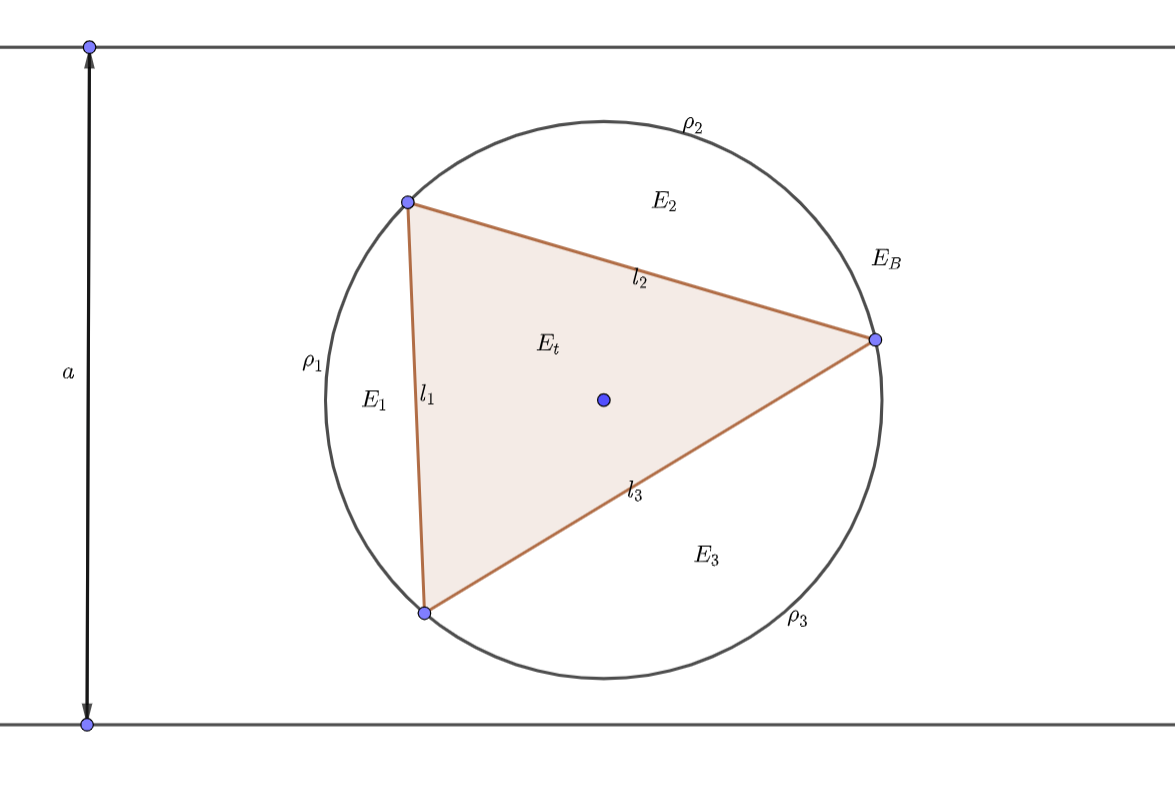
\includegraphics[width=0.8\textwidth]{figure.png}
}
% 表格模板
\renewcommand\arraystretch{0.8} % 设置表格高度为原来的0.8倍
\begin{table}[!htbp] % table标准
    \centering % 表格居中
    \begin{tabular}{p{1cm}<{\centering}p{1cm}<{\centering}p{3cm}<{\centering}p{5cm}<{\centering}} % 设置表格宽度
    %\begin{tabular}{cccc}
        \toprule
        $x_i$ & $f[x_1]$ & $f[x_i,x_{i+1}]$ & $f[x_i,x_{i+1},x_{i+2}]$ \\
        \midrule
        $x_0$ & $f(x_0)$ &                  &                          \\
        $x_0$ & $f(x_0)$ & $f'(x_0)$        &                          \\
        $x_0$ & $f(x_1)$ & $\frac{f(x_1)-f(x_0)}{x_1-x_0}$ & $\frac{f(x_1)-f(x_0)}{(x_1-x_0)^2}-\frac{f'(x_0)}{x_1-x_0}$\\
        \bottomrule
    \end{tabular}
\end{table}

\def\Log{\text{Log}} % 一个简单的宏定义
$\Log$ % 调用方法
\fi

\end{document}